%%%%%%%%%%%%%%%%%%%%%%%%%%%%%%%%%%%%%%%%%%%%%%%%%
%    			Hochschule Heilbronn			%
%			Modeling and Simulation			    %
% Materials Characterisation Report Template    %
%%%%%%%%%%%%%%%%%%%%%%%%%%%%%%%%%%%%%%%%%%%%%%%%%
% CHANGES                                       %
%   -Updated to use Helvetica font              %
%%%%%%%%%%%%%%%%%%%%%%%%%%%%%%%%%%%%%%%%%%%%%%%%%



\documentclass[twoside,10pt,a4paper]{article}
%describes the document we are making

%%%%%%%%%%%%%%%%%%%%%%%%%%%%%%%%%%%%%%%% 
%Document preamble, adds useful packages and sets up the document. 


%FONT AND TYPESETTING
\usepackage[ngerman]{babel}							%makes latex aware of your language, so better hyphenating etc
\usepackage[T1]{fontenc} 							%use the T1 for proper searching and use of ligatures etc
\usepackage[utf8]{inputenc}							%use UTF8 encoding for reading source code
\usepackage{helvet}								%use the helvetica font. This is very similar to the Arial font used in the Office templates.
\renewcommand{\familydefault}{\sfdefault}
\usepackage{microtype}								%enables microtypesetting
\usepackage{blindtext}
\usepackage{csquotes}

%PAGE LAYOUT
\usepackage[onehalfspacing]{setspace}				%adjusts linespacing
\usepackage{geometry}				                %adjusts page layout including margins
\usepackage{fancyhdr}
\geometry{left=2.5cm,right=2.5cm,top=3cm,bottom=3cm}	%the page geometry as defined, A4=210x297mm
\pagestyle{fancy}						            %includes page number in centred in footer
\fancyhf{}
\fancyhead[LE,LO]{Hochschule Heilbronn\\MMR}
\fancyhead[CE,CO]{Wärmeleitung mit\\alternativem Differenzenstern}
\fancyhead[RE,RO]{Prof. M.Scholle}
\fancyfoot[CE,CO]{\thepage}
\fancyfoot[LE,LO]{Fabian Reinwald}
\fancyfoot[RE,RO]{\today}
\renewcommand{\footrulewidth}{1pt}

%MATHS
\usepackage{mathtools} 								%for the rendering of maths
\numberwithin{equation}{section}					%reset numbering within a structural object
\numberwithin{figure}{section}						%reset numbering within a structural object

%SCIENCE
\usepackage[version=4]{mhchem}						%typesetting of chemical formulae
\usepackage{siunitx}								%typesetting of units and quantities with uncertainties etc
\sisetup{detect-all, detect-weight=true, detect-family=true}  %  if the rest of the text is bold the units will be as well
\sisetup{range-units=single}  						% don't include units in both parts of an \SIrange 
\sisetup{multi-part-units=single}					% don't repeat units for multi-part numbers such as numbers with uncertainties
\sisetup{separate-uncertainty}						%list values with uncertanties as X\pm Y rather than X(Y).

%FIGURES AND TABLES
\usepackage{caption}
\usepackage{graphicx}								%for the rendering of floating graphics
\usepackage[section]{placeins}						%defines float barriers at the end of sections. Set option [section] for this.
\usepackage{array} 								%for creating tables
\usepackage{booktabs}								%professional looking tables, provides /toprule etc
\usepackage{multicol}
\usepackage{float}
\usepackage{hyperref}



%BIBLIOGRAPHY
\usepackage[backend=biber,citestyle=numeric-comp,bibstyle=numeric,sorting=none,url=false,eprint=false,isbn=true,doi=true]{biblatex}
\addbibresource{./example.bib}	%the absolute or relative path of your bibliography file.
\usepackage{hyperref, bookmark}						%turns the references and citations into hyperlinks. This needs to be last on the preamble.
\hypersetup{colorlinks=true,linkcolor=black,citecolor=blue,urlcolor=blue}

%%%%%%%%%%%%%%%%%%%%%%%%%%%%%%%%%%%%%%%%%%%%%%%%%%%%%%%%


\begin{document}
%	Put the document stuff in here!
\fontfamily{phv}\selectfont
\begin{titlepage}			%makes a title page. Remember to change the author, CID, username and group number to what is appropriate for you!
\begin{figure}[h]
    \flushright
    
\includegraphics[height=1cm]{bilder/hhn.png}
\end{figure}
	\centering
	{\scshape\LARGE Hochschule Heilbronn\par}
	{\scshape \LARGE Modeling and Simulation\par}
	\vspace{0.5cm}
    \begin{figure}[h]
        \centering
        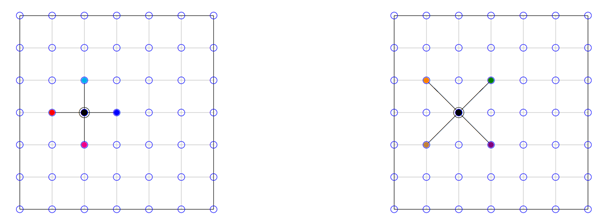
\includegraphics[width=\textwidth]{bilder/Picture1.png}
        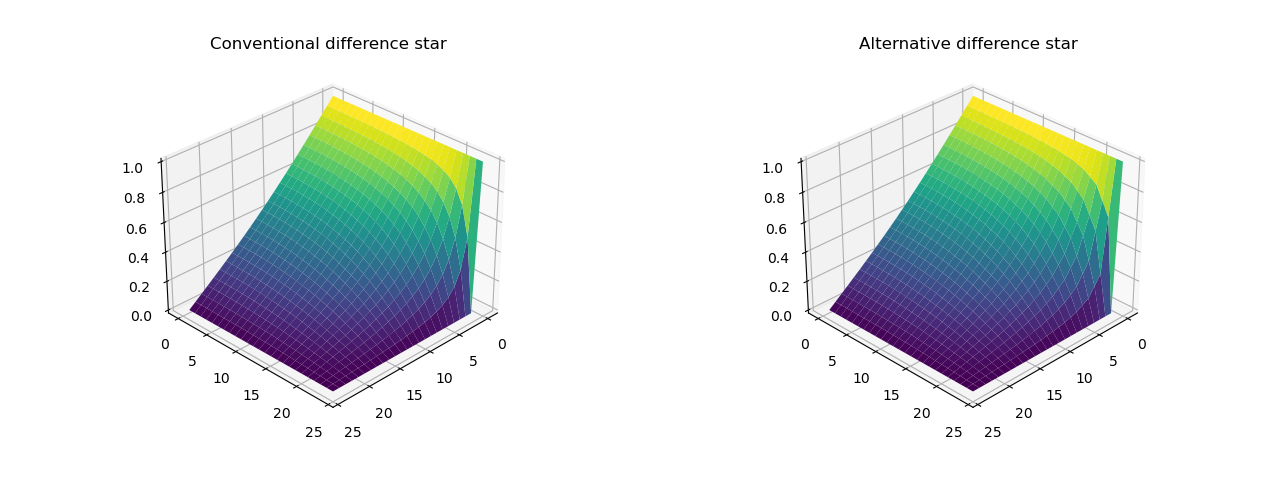
\includegraphics[width=\textwidth]{bilder/convalt.jpg}
    \end{figure}
	{\huge\bfseries Wärmeleitung mit alternativem Differenzenstern\par}
	\vspace{0.5cm}
	{\Large\itshape Fabian Reinwald\par}		%remember to change these!
	\vspace{0.5cm}
	%		{\large Group \@group\unskip\strut\par}
	{\large  Betreuer: Prof. M. Scholle \hfill Zeitraum: WS 2020/21\par}		%remember to change these!
	\vspace{0.5cm}
	{\large \today\par}
\end{titlepage}

\tableofcontents
\newpage
\section{Aufgabenstellung}
Das Standard-Verfahren zur Lösung der 2D Laplace-Gleichung basiert auf einer Mittelwertbildung der Werte der ’direkten Nachbarn’, so wie auf dem Titelbild links veranschaulicht. Dabei werden als ’direkte Nachbarn’ aber nur diejenigen in horizontaler und vertikaler Richtung angesehen, woraus der bekannte ’Differenzenstern’ in Form eines Plus-Zeichens resultiert.\\
Was aber ist mit den ’diagonalen Nachbarn’? Könnte man nicht auch ein alternatives Verfahren, so wie auf dem Titelbild rechts angedeutet, allein mit den diagonalen Nachbarn mit einem X-förmigen Differenzenstern verwenden?\\
Ziel der Aufgabe ist es, genau dies zu testen und z.B. auf das in der Vorlesung behandelte Wärmeleitproblem anzuwenden und mit den vorherigen Ergebnissen zu vergleichen.


\section{Einleitung}\label{sec:section1}
Um das stationäre Problem der Temperaturverteilung über einen 2-dimensionalen Bereich numerisch lösen zu können, muss das Gebiet in eine Menge von Knotenpunkten unterteilt werden. Mit einer finiten Differenzenmethode kann nun ein Temperaturverlauf ermittelt werden und es wird kein analytisches Lösen einer Laplacegleichung benötigt.
Für diese Differenzen wird ein „Differenzenstern“ verwendet wie er in Abbildung \ref{fig:1} zu sehen ist.

    \begin{figure}[h]
        \centering
        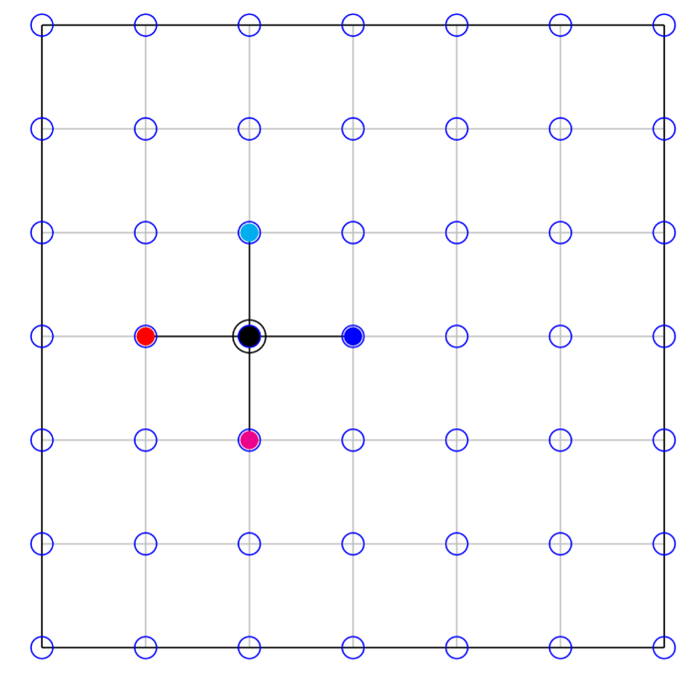
\includegraphics[width=8cm]{bilder/Picture2.png}
        \caption{Konventioneller Differenzenstern direkter Nachbarn in einem diskretisiertem Gebiet}
        \label{fig:1}
    \end{figure}

Um nun den mittleren Wert zu bestimmen, lässt sich einfach der Mittelwert der vier markierten angrenzenden Punkte berechnen.
Nun ist es nicht unbedingt notwendig genau diese vier Punkte zu verwenden, stattdessen kann man auch die vier diagonal angrenzenden Punkte verwenden, was einen um 45° rotiertes Differenzenstern ergibt wie in \ref{fig:2} zu sehen.

    \begin{figure}[h]
        \centering
        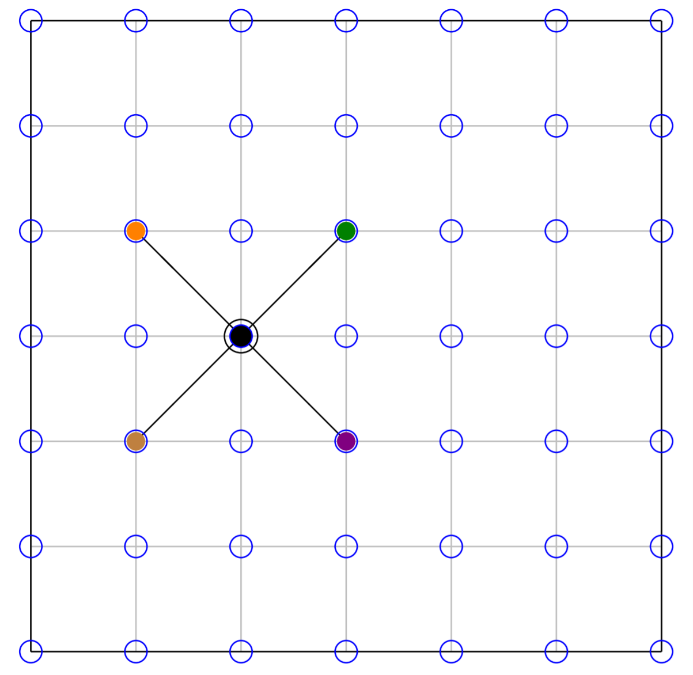
\includegraphics[width=8cm]{bilder/Picture3.png}
        \caption{Alternativer Differenzenstern diagonaler Nachbarn in einem diskretisiertem Gebiet}
        \label{fig:2}
    \end{figure}


\section{Diskretisierung des Laplace-Operators}
Rein instinktiv würde man nun davon ausgehen, dass der Mittelpunkt weiterhin vom Mittelwert der vier angrenzenden Punkte berechnet wird. Um dies jedoch zu beweisen muss der Laplace-Operator der Wärmeleitung per Taylor diskretisiert werden.
Der Vollständigkeit halber wird hier auch die Diskretisierung des bisherigen Verfahrens dargestellt. Eine ausführlichere Version findet sich in den \href{https://ilias.hs-heilbronn.de/goto.php?target=file_137931_download&client_id=iliashhn}{Lecture Notes} des Modeling and Simulation Kurses.\\
Der Laplace-Operator der Wärmeleitung in zwei Dimensionen mit T=T(x,y):
\begin{equation}\label{laplace}
\\
    \nabla ^2 T=\frac{\partial^2 T}{\partial x^2}+\frac{\partial^2 T}{\partial y^2}=0
\\
\end{equation}
Das vollständige Verständnis dieser Funktion ist für die numerische Lösung nicht erforderlich. Allerdings müssen nun für die beiden partiellen Ableitungen entsprechende Gleichungen gefunden werden. Dafür wird angenommen, dass sich die Temperatur linear zwischen denen von uns festgelegten Gitterpunkten ändert. Nun betrachtet man die Punkte zwischen diesen Gitterpunkten um Gleichungen für eine partielle Ableitung aufzustellen.
\\

\begin{multicols}{2}
\textit{Konventionell:}\\
\begin{equation}
    \left.\frac{\partial T}{\partial x}\right|_{i-\frac{1}{2},j}=\frac{T_{i,j}-T_{i-1,j}}{\Delta x}
\end{equation}
\textit{Alternativ:}\\
\begin{equation}
    \left.\frac{\partial T}{\partial x}\right|_{i-\frac{1}{2},j}=\frac{T_{i,j}-\frac{1}{2}(T_{i-1,j+1}+T_{i-1,j+1})}{\Delta x}
\end{equation}
\end{multicols}

\begin{multicols}{2}
\begin{equation}
    \left.\frac{\partial T}{\partial x}\right|_{i+\frac{1}{2},j}=\frac{T_{i+1,j}-T_{i,j}}{\Delta x}
\end{equation}
\begin{equation}
    \left.\frac{\partial T}{\partial x}\right|_{i+\frac{1}{2},j}=\frac{\frac{1}{2}(T_{i+1,j+1}+T_{i+1,j-1})-T_{i,j}}{\Delta x}
\end{equation}
\end{multicols}
Dabei wird bei beiden Verfahren gleich vorgegangen: Für die Ableitung am Punkt T(i+$\frac{1}{2}$,j) wird die Differenz von T(i,j) und T(i-1,j) durch die Schrittweite $\Delta$x geteilt. Mit dem gedreheten Stern muss der Punkt T(i-1,j) erst mit Hilfe der gegebenen Punkte hergeleitet werden. Dafür werden die angrenzenden Punkte arithmetisch gemittelt. Dieser Vorgang ist in Abbildung \ref{fig:3} veranschaulicht.

    \begin{figure}[H]
        \centering
        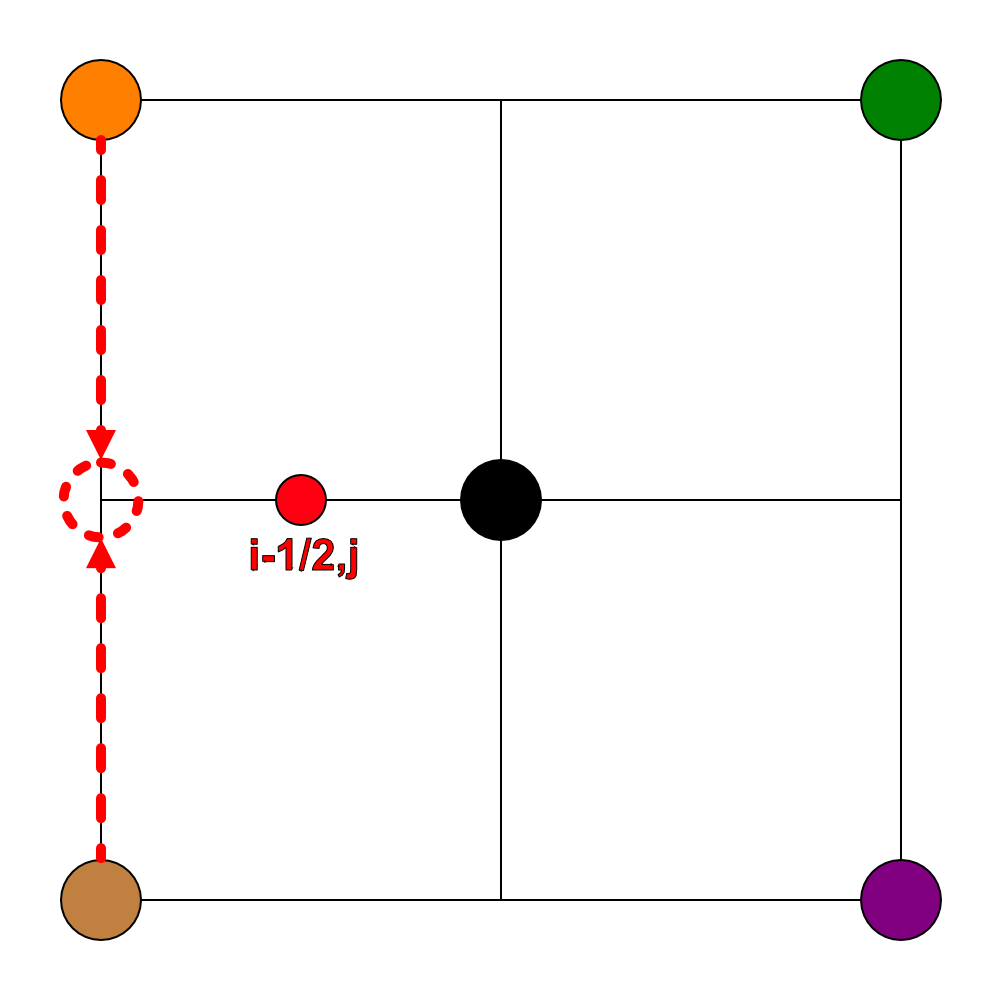
\includegraphics[width=8cm]{bilder/xstar.png}
        \caption{Herleiten eines 'virtuellen' Punktes zur Berechnung der partiellen Ableitung}
        \label{fig:3}
    \end{figure}
 Dieser Vorgang wird nun für die y-Richtung wiederholt.
 \begin{multicols}{2}

\begin{equation}
    \left.\frac{\partial T}{\partial y}\right|_{i-\frac{1}{2},j}=\frac{T_{i,j}-T_{i,j-1}}{\Delta y}
\end{equation}
 \\
\begin{equation}
    \left.\frac{\partial T}{\partial y}\right|_{i-\frac{1}{2},j}=\frac{T_{i,j}-\frac{1}{2}(T_{i-1,j-1}+T_{i+1,j-1})}{\Delta y}
\end{equation}
\end{multicols}

 \begin{multicols}{2}

\begin{equation}
    \left.\frac{\partial T}{\partial y}\right|_{i+\frac{1}{2},j}=\frac{T_{i,j+1}-T_{i,j}}{\Delta y}
\end{equation}
 \\
\begin{equation}
    \left.\frac{\partial T}{\partial y}\right|_{i+\frac{1}{2},j}=\frac{\frac{1}{2}(T_{i-1,j+1}+T_{i+1,j+1})-T_{i,j}}{\Delta y}
\end{equation}
\end{multicols}

Mit der Annahme, dass die Temperaturgradienten linear zwischen den Knoten verlaufen, dann gilt:
\begin{equation}
    \left.\frac{\partial^2 T}{\partial x^2}\right|_{i,j}=\frac{\left.\frac{\partial T}{\partial x}\right|_{i+\frac{1}{2},j}-\left.\frac{\partial T}{\partial x}\right|_{i-\frac{1}{2},j}}{\Delta x}
\end{equation}
Durch Einsetzen der obigen Gleichungen ergibt sich jeweils (analog in y-Richtung):\\
\textit{Konventionell:}\\
\begin{equation}
    \left.\frac{\partial^2 T}{\partial x^2}\right|_{i,j}=\frac{T_{i+1,j}+T_{i-1,j}-2T_{i,j}}{\Delta x^2}
\end{equation}
\begin{equation}
    \left.\frac{\partial^2 T}{\partial y^2}\right|_{i,j}=\frac{T_{i,j+1}+T_{i,j-1}-2T_{i,j}}{\Delta y^2}
\end{equation}
\textit{Alternativ:}\\
\begin{equation}
    \left.\frac{\partial^2 T}{\partial x^2}\right|_{i,j}=\frac{\frac{1}{2}(T_{i+1,j+1}+T_{i+1,j-1}+T_{i-1,j+1}+T_{i-1,j-1})-2T_{i,j}}{\Delta x^2}
\end{equation}
\begin{equation}
    \left.\frac{\partial^2 T}{\partial y^2}\right|_{i,j}=\frac{\frac{1}{2}(T_{i+1,j+1}+T_{i+1,j-1}+T_{i-1,j+1}+T_{i-1,j-1})-2T_{i,j}}{\Delta y^2}
\end{equation}
Auffällig ist hier, dass beim konventionellen Differenzenstern jeweils nur zwei der Nachbarpunkte in pro Dimension einfließen. Bei der alternativen Methode hingegen werden alle benachbarten Punkte benötigt.
Setzt man die obigen Gleichungen nun in die anfangs gegebene Laplace-Gleichung (\ref{laplace}) ein und stellt diese nach T(i,j) um, so erhält man eine Formel zur Bestimmung des Mittelwert des Kreuzes mit Hilfe der angrenzenden Punke - eben mit finiten Differenzen.\\
\textit{Konventionell:}\\
\begin{equation}
    T_{i,j}=\frac{1}{4}(T_{i+1,j}+T_{i-1,j}+T_{i,j+1}+T_{i,j-1})
\end{equation}
\textit{Alternativ:}\\
\begin{equation}\label{solution}
    T_{i,j}=\frac{1}{4}(T_{i+1,j+1}+T_{i+1,j-1}+T_{i-1,j+1}+T_{i-1,j-1})
\end{equation}
Die Gleichung (\ref{solution}) zeigt, dass unsere anfängliche Überlegung korrekt war und der Punkt T(i,j) weiterhin durch das arithmetische Mittel der angrenzenden Punkte beschrieben werden kann. Dieser Aspekt lässt sich nun ohne Probleme in ein Python Programm implementieren.

\section{Diskretisierung einer homogenen Neumann-Randbedingung}
Nun muss noch eine genauere Betrachtung der Neumann-Randbedingung erfolgen, diese besagt, dass die Ableitung des Feldes an der Grenze Null beträgt. Doch wie kann man dieses Problem lösen ohne Punkte auserhalb des Feldes zu Rate zu ziehen (welche nicht existieren).\\
Bei der konventionellen Methode befindet sich an einer Grenze immer einer der vier Punkte außerhalb, dieser wird nun nach innen 'gespiegelt' indem man den Punkt gegenüber von ihm doppelt zählt.
Bei dem um 45° gedrehten Stern befinden sich nun sogar zwei Punkte außerhalb, aus Symmetriegründen verdoppelt man nun die verbleibenden zwei Punkte um dies auszugleichen.
An der Grenze T(0,0:N-1) sähe die Formel für T(0,j) nun wie folgt aus:\\
\begin{equation}
    T_{0,j}=\frac{1}{4}(2T_{1,j-1}+2T_{1,j+1})
\end{equation}
Auch dieser Aspekt lässt sich für beliebige Seiten in ein Python Programm implementieren.

\section{Implementierung in Python}
Ein Python Programm welches die beiden Verfahren vergleicht ist entweder diesem Dokument beigelegt oder ist ansonsten auf \href{https://github.com/FReinwald/Heat-transfer-with-alternative-difference-star}{Github} zu finden.

\section{Vergleich der Differenzensterne}
Eine Betrachtung der erzeugten Plots zeigt, dass auch der gedrehte Differenzenstern eine numerische Lösung möglich macht. Auf den ersten Blick erscheinen die Ergebnisse auch sehr ähnlich wie in \ref{fig:compare} zu sehen. Da stellt sich jetzt die Frage warum man in Literatur oder Anwendungen nicht zu Gesicht bekommt. Dafür gibt es verschiedene plausible Gründe.
\begin{figure}[h]
        \centering
        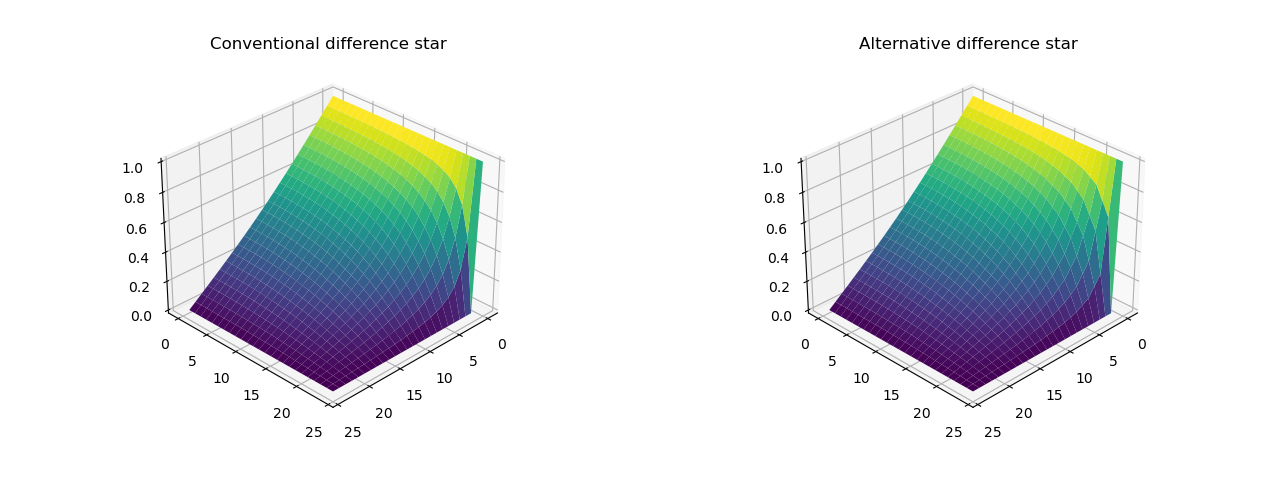
\includegraphics[width=\textwidth]{bilder/convalt.jpg}
        \caption{Darstellung des Temperaturverlauf mit konventionellem und alternativem Differenzenstern}
        \label{fig:compare}
    \end{figure}
\subsection{Intuition}
Vermutlich eines der besten Argumente gegen den X-Stern ist, dass er nicht intuitiv für den Anwender ist. Weshalb sollte er einen Stern über sein Feld wandern lassen, welcher um 45° zu diesem gedreht ist? Die etablierte Methode lässt sich da deutlich leichter nachvollziehen, da die verwendeten Felder auch wirklich einen direkten Kontakt zum Gesuchten haben.

\subsection{Rechenperformance}
Wie im Python Skript zu sehen braucht der X-Stern zwar weniger Rechenschritte als der +-Stern, für diese aber so viel länger, dass er insgesamt langsamer ist. Bei numerischen Lösungen ist die recheneffizienz sehr wichtig wenn die Modelle größer und genauer werden.

\subsection{Modellperformance}
Im Vergleich zum +-Stern sieht in Abbildung \ref{fig:relative} man beim X-Stern Abweichungen von bis zu 25(\%), gerade bei starken Temperaturänderungen. Natürlich könnte man nun im Detail analysieren welches der beiden Modelle genauer ist und näher an die Realität herankommt - allerdings lässt sich dies auch logisch erklären ohne die exakte Lösung zu kennen. Denn gerade zwei Aspekte müssen den X-Stern an sich automatisch zum schlechteren Modell als den konventionellen Differenzenstern machen.\\
\begin{figure}[H]
        \centering
        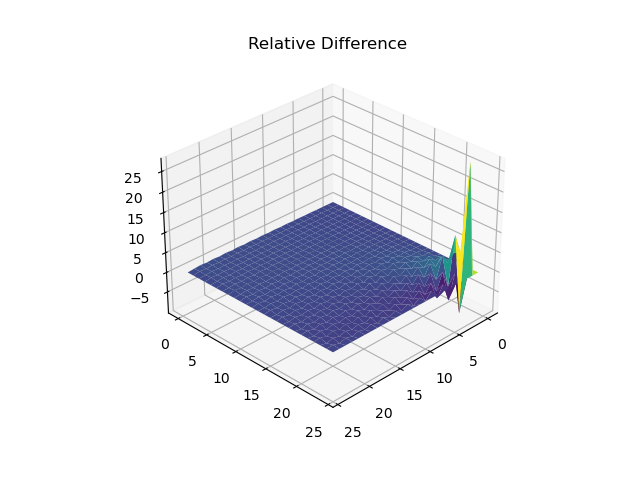
\includegraphics[width=\textwidth]{bilder/rel diff 2.png}
        \caption{Relative Abweichung des alternativen Differenzenstern zum Konventionellen}
        \label{fig:relative}
    \end{figure}
\subsubsection{Abstand der Nachbarpunkte}
Bei unserem X-förmigen Stern sind die benachbarten Punkte, welche wir zur Berechnung verwenden um ca. 40(\%) weiter vom Zentrum entfernt. Dies ist der Geometrie des Gitters geschuldet. Bei einem Abstand von 1 der Punkte, so ist der Abstand beim +-Stern weiterhin 1, aber beim X-Stern verwenden wir Punkte mit einem Abstand von $\sqrt{2}$.
\subsubsection{Ecken des Felds}
Um einen Wert in der Ecke des Feldes berechnen zu können, so befinden sich beim +-Stern zwei der vier Punkte auserhalb des Feldes, was noch durch Verdoppelung der restlichen zwei Punkte ausgeglichen werden kann.\\
Bei unserem X-Stern befinden sich stattdessen drei der vier Punkte außerhalb, was nicht ausgeglichen werden kann. Somit muss die Performance dieser Randwerte als schlecht angesehen werden, was sich auch auf das restliche Feld auswirkt.
\subsection{Fazit}
Zusammengefasst lässt sich sagen, dass ein gedrehter Differenzenstern zwar ein akzeptables Ergebnis liefert, die herkömmliche Methode aber zu bevorzugen ist und zu Recht deutlich populärer ist.

\end{document}